\begin{figure}[h]
%\centering
	\begin{subfigure}[b]{0.25\textwidth}
		\centering
		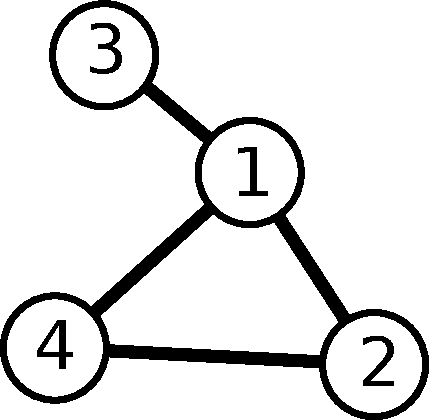
\includegraphics[width=\textwidth]{pix/simple_graph.pdf}
		\caption{Simple graph}
		%\label{fig:gull}
	\end{subfigure}
	\hfill
	\begin{subfigure}[b]{0.25\textwidth}
		\raggedright
		\qquad \begin{description} \itemsep -0.5em
			\item[1:] 2, 3, 4
			\item[2:] 1, 4
			\item[3:] 1
			\item[4:] 1, 2
		\end{description}
		\caption{Adjacency list}
		%\label{fig:gull}
	\end{subfigure}
	\hfill
	\begin{subfigure}[b]{0.25\textwidth}
		\centering
		$\begin{matrix}
			0&1&1&1\\ 1&0&0&1 \\ 1&0&0&0 \\ 1&1&0&0
		\end{matrix}$
		\caption{Adjacency matrix}
		%\label{fig:gull}
	\end{subfigure}
	%\hfill
\caption{Graph representation examples}\label{fig:graphexamples}
\end{figure}